%Paul E. West

%\documentclass[xcolor=svgnames]{beamer}
\documentclass{beamer}
\usepackage[boxed,vlined,figure]{algorithm2e}

%\usecolortheme[named=FireBrick]{structure}
%\usecolortheme[named=black]{structure}
%\usecolortheme{beetle}
%\usecolortheme{beaver}
%\usecolortheme{crane}
%\usecolortheme{dolphin}
%\usecolortheme{dove}
%\usecolortheme{fly}
%\usecolortheme{lily}
\usecolortheme{orchid}
%\usecolortheme{rose}
%\setbeamercolor{background canvas}{bg=Gold!25}
%\setbeamercolor{background canvas}{bg=Black!100}
%\setbeamercolor{foreground}{bg=Gold!25}
%\setbeamercolor{normal text}{fg=green,bg=black}
%\setbeamercolor*{palette primary}{use=structure,fg=green,bg=black} 
\mode<presentation>{
    \usetheme{Darmstadt}
    \setbeamercovered{invisible}
    %\setbeamercovered{transparent}
    \setbeamercolor*{palette primary}{use=structure,fg=white,bg=blue}
    \setbeamercolor*{palette secondary}{use=structure,fg=white,bg=blue}
    \setbeamercolor*{palette tertiary}{use=structure,fg=white,bg=blue}
}

\usepackage[english]{babel}
\usepackage[latin1]{inputenc}
\usepackage{times}
\usepackage[T1]{fontenc}
%\usepackage{epsfig}
\usepackage{ulem}
\usepackage{color,soul}

\usepackage{graphicx}
\usepackage{amssymb}
\usepackage{url,hyperref}
\definecolor{beamer@blendedblue}{rgb}{1,.6,.2}
%\usepackage{tikz}
%\usetikzlibrary{shapes}
%\usetikzlibrary{arrows}
%\tikzstyle{block}=[draw opacity=0.7, line width=1.4cm]
\usepackage{listings}
\lstset{language=Java}
\lstset{showspaces=false}
\lstset{showstringspaces=false}
\lstset{tabsize=4}
\lstset{basicstyle=\tiny}


%\usecolortheme[overlystylish]{albatross}
%\usecolortheme[]{lily}
%\usecolortheme[]{albatross}
%\usecolortheme[]{orchid}
%\setbeamercolor{normal text}{fg=green!10}

\title{CSCI 315: Data Structures \\ 
    Basic Unix Commands
}
\author{Paul E. West, PhD}

\institute{
  Department of Computer Science\\
  Charleston Southern University
}

\subject{Software Programming}
%\keywords{Performance Counters, Multicore}

%\pgfdeclareimage[height=1.0cm]{university-logo}{../imgs/csu-logo}
\pgfdeclareimage[height=0.75cm]{university-logo}{../imgs/csu-logo}
%\pgfdeclareimage[height=0.50cm]{university-logo}{../imgs/csu-logo}
\logo{\pgfuseimage{university-logo}}

\begin{document}

\begin{frame}
  \titlepage
\end{frame}

\section{Introduction}
\subsection{}
\begin{frame}{}
\begin{itemize}
\item Although modern Linux is equipped with a \textit{fancy schmancy} Graphical User Interface (GUI), for system administrators (and *\textit{real}* programmers), shell is the best tool to handle everything.
\item In GUI mode, you can activate our shell by opening a terminal window.
\item The terminal window is your control panel for the system.
\end{itemize}
\end{frame}

\begin{frame}{Opening a terminal}
\begin{columns}[c]
\column{0.50\textwidth}
\begin{itemize}
\item Terminal window shows a standard prompt
\item Prompts displays all kinds of information, but they are not part of the commands you are giving to your system.
\end{itemize}
\column{0.50\textwidth}
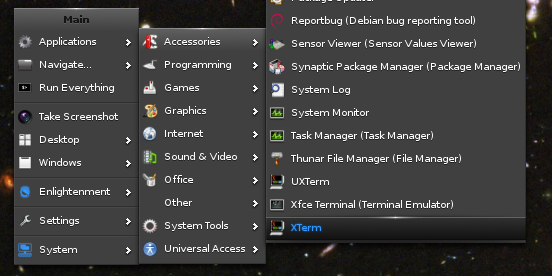
\includegraphics[width=1.0\textwidth]{../imgs/terminal-open.png} \\
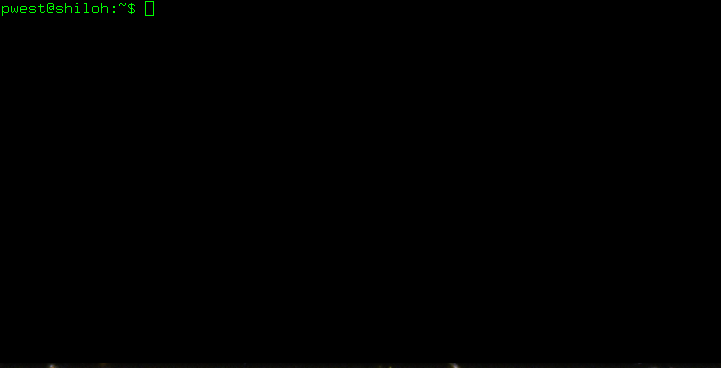
\includegraphics[width=1.0\textwidth]{../imgs/terminal.png}
\end{columns}
\end{frame}

\section{Text Editors}
\subsection{}

\begin{frame}{Choosing a Text Editor}
\begin{itemize}
\item Do take some time to choose a good text editor.
\begin{itemize}
\item You will be using it a lot.
\end{itemize}
\item Most Windows/OSX editors have a clone in Linux.
\item Linux has numerous choices.
\item Be aware that text editors can become a religous affair...
\end{itemize}
\end{frame}

\begin{frame}{vi}
\begin{columns}
\column{0.50\textwidth}
\begin{itemize}
\item Light weight with a high learning curve
\item A \textit{fast} editor once you learn it
\item :q to quit from vi
\item :wq  to write the change to the file
\item :q! quit without saving changes
\item To exit from editing mode, click esc key
\item i to insert
\item x to delete a char
\end{itemize}
\column{0.50\textwidth}
\begin{itemize}
\item dd to delete a line
\item / text search
\item same on every machine
\end{itemize}

\includegraphics[width=1.0\textwidth]{../imgs/meme-5393808378298368.png}
\end{columns}
\end{frame}

\begin{frame}{emacs}
\begin{itemize}
\item Lots of features -- tons of capabilities
\item LISP
\item Your hand may be warpped from all the hotkeys
\item Not always the same on every machine
\end{itemize}
\begin{center}
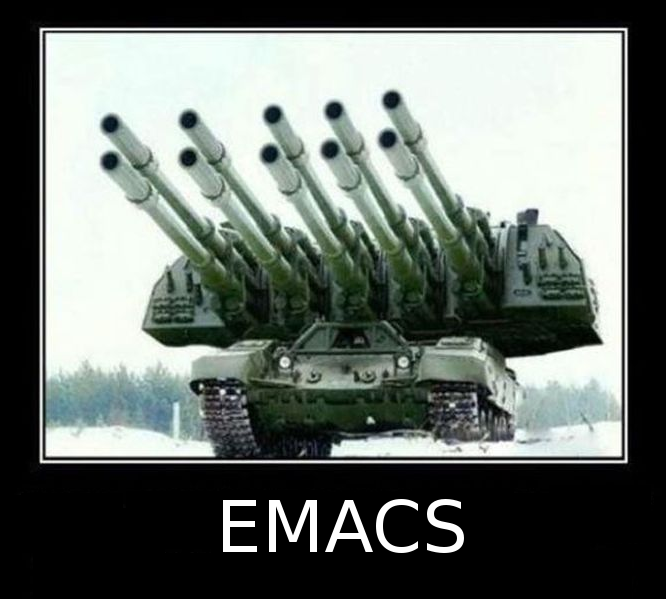
\includegraphics[width=0.4\textwidth]{../imgs/emacs.png}
\end{center}
\end{frame}

\begin{frame}{nano}
\begin{itemize}
\item simple!
\item commands are at the bottom of your screen
\item same on every machine
\end{itemize}
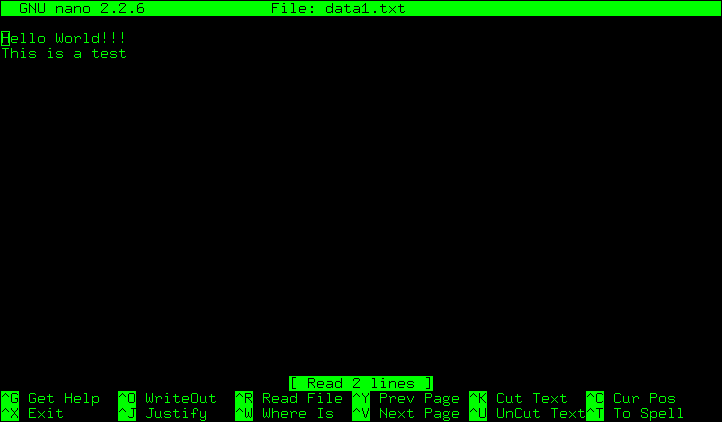
\includegraphics[width=0.8\textwidth]{../imgs/nano.png}
\end{frame}

\begin{frame}{Don't Be That Guy}

\includegraphics[width=0.8\textwidth]{../imgs/meme-5660755493912576.png}
\end{frame}

\begin{frame}{Graphical Text Editors}
\begin{itemize}
\item gvim: graphical vim
\item xemacs: graphical emacs
\item gedit: like MS wordpad/notepad
\item atom: more advance text editor
\item sublime: newer, very powerful
\item kate: KDE text editor
\item tea: Minimal QT text editor
\item jed: Very basic.  Essentiall nano++
\end{itemize}
\end{frame}

\section{Commands}
\subsection{}
\begin{frame} {ls}
\begin{itemize}
\item ls (list)
\begin{itemize}
\item displays a list of files in the current working directory, like dir in DOS
\end{itemize}
\item -a 
\begin{itemize}
\item display hidden (start with a '.') files
\end{itemize}
\item -A
\begin{itemize}
\item Do not display '.' and '..'
\item '.' means current directory
\item '..' means upper layer directory
\end{itemize}
\item -l
\begin{itemize}
\item display file lists with long format
\end{itemize}
\item -s
\begin{itemize}
\item display file size
\end{itemize}
\item -h
\begin{itemize}
\item display sizes in a more human readable format
\end{itemize}
\end{itemize}
\end{frame}

\begin{frame}{cd}
\begin{itemize}
\item change directory
\item cd /usr/bin
\begin{itemize}
\item Change directory to /usr/bin directory
\end{itemize}
\item cd ..
\begin{itemize}
\item Change to upper layer directory
\end{itemize}
\item cd /
\begin{itemize}
\item Change to root directory
\end{itemize}
\item cd ~
\begin{itemize}
\item Change to user home directory
\end{itemize}
\end{itemize}
\end{frame}

\begin{frame}{Directory Operations}
\begin{itemize}
\item mkdir
\begin{itemize}
\item Make directory
\item mkdir temp
\item mkdir temp2
\item mkdir temp/insideTemp
\end{itemize}
\item rmdir
\begin{itemize}
\item remove directory
\item rmdir temp2
\end{itemize}
\end{itemize}
\end{frame}

\begin{frame}{Creating a file with cat}
cat is a command we will discuss later\\
gedit, vi, and nano are text editors available in our Linux and either can be used to create a file as well.
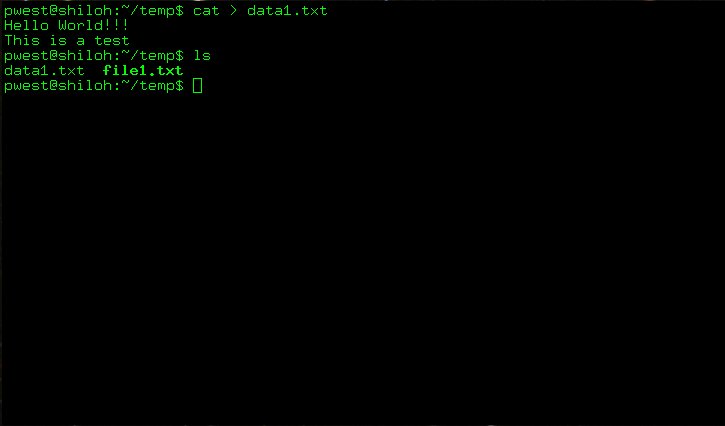
\includegraphics[width=1.0\textwidth]{../imgs/file-create.png} \\
\end{frame}

\begin{frame}{File Operations: cp}
\begin{itemize}
\item copy
\item cp data1.txt data2.txt
\item cp data3.txt temp
\begin{itemize}
\item -i
\end{itemize}
\item ask before overwrite
\begin{itemize}
\item -v 
\end{itemize}
\item display copying process
\begin{itemize}
\item -R
\end{itemize}
\item recursive copy, including sub-directories
\item cp -R * backup
\end{itemize}
\end{frame}

\begin{frame}{File Operations: rm}
\begin{itemize}
\item rm
\begin{itemize}
\item remove file or directory
\item rm data1.txt
\item rm *
\item -f
\begin{itemize}
\item force remove files
\item rm -f *.txt
\end{itemize}
\item -r
\begin{itemize}
\item recursive remove files, including sub-directories
\item rm -r *
\end{itemize}
\item -v
\begin{itemize}
\item display removing process
\end{itemize}
\end{itemize}
\end{itemize}
\end{frame}

\begin{frame}{Directory Usage}
\begin{itemize}
\item Any command that accepts a file as a parameter assumes that file is in the present (current) working directory (pwd) unless told otherwise.
\item Use relative or absolute paths to indicate where a file is.
\item Absolute paths start with a / and the path begins from the highest level
\item Relative paths NEVER start with a / and are how to get to the file from the pwd
\item .. Is your parent directory, useful in relative paths
\end{itemize}
\end{frame}

\begin{frame}{More File Operations}
\begin{itemize}
\item mv
\begin{itemize}
\item move files or rename a file
\item mv data1.txt ..
\item mv data1.txt data4.txt
\end{itemize}
\item pwd
\begin{itemize}
\item print (present) working directory
\end{itemize}
\item file
\begin{itemize}
\item display file type
\item file filename
\item file *
\end{itemize}
\end{itemize}
\end{frame}

\begin{frame}{Even More File Operations}
\begin{itemize}
\item head
\begin{itemize}
\item head shows the first few lines of a file
\item head data1.txt shows first 10 lines of data1.txt
\item head -20 data1.txt shows first 20 lines
\end{itemize}
\item tail
\begin{itemize}
\item tail shows the last few lines of a file
\item tail data1.txt shows last 10 lines of data1.txt
\item -r : show content in reverse order
\end{itemize}
\item wc
\begin{itemize}
\item word count
\item 1st column -> number of lines
\item 2nd column -> number of unique words
\item 3rd column -> total word counts
\end{itemize}
\end{itemize}
\end{frame}

\begin{frame}{Yes, Even More File Operations}
\begin{itemize}
\item find
\begin{itemize}
\item -name	filename you are looking for
\item -print	output results
\item find /usr -name compress -print
\end{itemize}
\item grep
\begin{itemize}
\item To search specified texts and display them
\item grep text files
\item more later
\end{itemize}
\item ln
\begin{itemize}
\item To link a file
\item ln -s data4.txt test
\item More later on linking
\end{itemize}
\end{itemize}
\end{frame}

\section{Redirect}
\subsection{}
\begin{frame}{Input/Output (I/O)}
\begin{itemize}
\item Three standard input/output devices
\begin{itemize}
\item \textit{stdin} <- keyboard input
\item \textit{stdout} <- Monitor output
\item \textit{stderr} <- Error output device
\end{itemize}
\end{itemize}
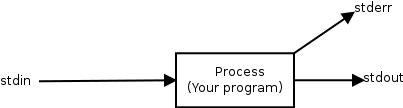
\includegraphics[width=0.8\textwidth]{../imgs/input-output.png}
\end{frame}

\begin{frame}{PIPE}
\begin{itemize}
\item Redirect output of one program to another
\item EX: \\
ls -al /etc | more
\end{itemize}

\includegraphics[width=0.8\textwidth]{../imgs/pipe-more.png} \\
\begin{itemize}
\item This can continue on...
\item What Data Structure does this look like?
\end{itemize}
\end{frame}

\begin{frame}{I/O Redirect to Files}
\begin{itemize}
\item Use < and > to redirect I/Os
\item cat > output.dat
\item Use Ctrl-d to quit
\item cat >> output.dat
\begin{itemize}
\item This will attach new texts to the end of output.dat (append)
\end{itemize}
\item cat !> output.dat
\begin{itemize}
\item will force overwrite output.dat
\end{itemize}
\end{itemize}
\end{frame}

\begin{frame}{Hey Look, Even \textit{More} File Operations!}
\begin{itemize}
\item more
\begin{itemize}
\item pausing output
\item ls -al | more
\end{itemize}
\item less
\begin{itemize}
\item hmmm, what does less do?
\end{itemize}
\item cat (concatenate)
\begin{itemize}
\item display file contents or concatenate a file to another
\item cat data1.txt | more
\item cat data1.txt >> data2.txt
\item cat data1.txt data2.txt >> data3.txt
\end{itemize}
\item tac
\begin{itemize}
\item hmmm, what does tac do?
\end{itemize}
\end{itemize}
\end{frame}

\begin{frame}{Printing}
\begin{itemize}
\item lp
\begin{itemize}
\item prints the named files to the printer
\item -d : specify the printer
\item -n how many copies
\end{itemize}
\item lpstat
\begin{itemize}
\item displays the status of print jobs sent to any printer with the lp command
\end{itemize}
\item cancel
\begin{itemize}
\item removes all of the specified jobs from printer queue
\end{itemize}
\end{itemize}
\end{frame}

\begin{frame}{Printing Continued}
\begin{itemize}
\item Some systems use different commands
\item lpr
\begin{itemize}
\item for printing
\item -P specify the printer
\item -\# number of copies
\item -m mail you when printing is done
\end{itemize}
\item lprm
\begin{itemize}
\item remove printing jobs
\item -P specify the printer
\end{itemize}
\end{itemize}
\end{frame}

\begin{frame}{Misc Commands}
\begin{itemize}
\item passwd (password)
\begin{itemize}
\item Change the password for the current user
\end{itemize}
\item man (manual pages)
\begin{itemize}
\item man ls
\end{itemize}
\item info (information of a command)
\begin{itemize}
\item info ls
\end{itemize}
\item --help (how to use a command)
\begin{itemize}
\item ls --help
\end{itemize}
\end{itemize}
\end{frame}

\section{Regex}
\subsection{}

\begin{frame}{Universal Characters}
\begin{itemize}
\item * - all possible combination(s)
\begin{itemize}
\item des* - desk, desktop, description, ...
\end{itemize}
\item ? - match exact position
\begin{itemize}
\item des? - desk, des9, ...
\end{itemize}
\item ls -al *.ps
\item cat ??go
\item more *a*b?
\item $[ ]$ - symbols in the quote
\begin{itemize}
\item ls -al $[$ms$]$oon means to list files of moon and soon
\item more $[$a-p$]$ount means to list files of aount, bount, count, ...,  pount
\end{itemize}
\end{itemize}
\end{frame}

\begin{frame}{Advanced grep Operations}
\begin{itemize}
\item Global or Get Regular Expression and Print
\item LEARN IT, it can save time
\item grep -hilnvw pattern filename
\item fgrep -hilnvwx string filename 
\begin{itemize}
\item Fixed grep, fast, only works with string
\end{itemize}
\item egrep -hilnvw pattern filename
\begin{itemize}
\item Extended grep, supports extended regular expression
\end{itemize}
\item Parameters:
\begin{itemize}
\item -n Print line number
\item -w Restricts matching to whole words only
\item -v displays all lines NOT matching
\item -l displays a list of the files that contain the specified pattern, useful when filename has wildcards
\item -x displays lines that are exactly equal to string
\end{itemize}
\end{itemize}
\end{frame}

\begin{frame}{Advanced grep Operations}
\begin{itemize}
\item cat > grepfile \\
Well, you know it's your bedtime, \\
So turn off the light, \\
Say all your prayers and then, \\
Oh you sleepy young heads dream of wonderful things, \\
And you will be swimming through the sea \\
\item grep the grepfile
\item grep -wn the grepfile
\item grep -v the grepfile
\end{itemize}
\end{frame}

\begin{frame}{Advanced grep Operations}
\begin{itemize}
\item grep .nd grepfile
\item grep $\hat{}$ .nd grepfile
\item grep sw*.ng grepfile
\item grep $[$A-D$]$ grepfile
\item grep a. grepfile
\end{itemize}
\end{frame}

\begin{frame}{Expressions}
\begin{itemize}
\item .	Matches any single character
\item $[]$ Matches any single characters enclosed in brackets.
\item If the first character after the $[$ is $\hat{}$ , then any character not enclosed in brackets is matched
\item * May follow any character and denotes zero or more occurrences of the character that precedes it.
\item $\hat{}$ Matches the beginning of a line only
\item \$ Matches the end of a line only
\end{itemize}
\end{frame}

\begin{frame}{Login and Logout}
\begin{itemize}
\item In GUI mode you can easily login and logout using mouse click
\item In text mode, you have to use command to logout a system.
\item After logout, do not power off the system!
\end{itemize}
\end{frame}

\begin{frame}{Shutdown}
\begin{itemize}
\item time
\begin{itemize}
\item hh:mm - shutdown 10:45
\item +m - shutdown +5
\item now - shutdown now
\end{itemize}
\item warning message
\begin{itemize}
\item shutdown +5 "system will shutdown in 5 minutes"
\end{itemize}
\item r - reboot after shutdown
\begin{itemize}
\item shutdown -r now
\item shutdown -r 23:50 \&
\end{itemize}
\item h - halt the system
\begin{itemize}
\item shutdown -h now
\item After seeing "system halted", you can power off the system.
\end{itemize}
\item c - cancel shutdown command
\begin{itemize}
\item shutdown -c
\end{itemize}
\end{itemize}
\end{frame}

\begin{frame}{Reboot}
\begin{itemize}
\item -n - no sync before reboot
\begin{itemize}
\item sync - to flush buffer and write them back to disks
\end{itemize}
\item -f - force reboot
\end{itemize}
\end{frame}

\begin{frame}{Man Page}
\begin{itemize}
\item The man command allows you to access the MANual pages for a UNIX command.
\item To get additional help on any of the commands listed below, you can always type man name\_of\_command at the command prompt.
\item Examples:\\
man ls \\
man cd
\end{itemize}
\end{frame}

\section{User Admin}
\subsection{}
\begin{frame}{Management Tools}
\begin{itemize}
\item User Management Tools
\item useradd- This command is used to add a new user account to the system. Its options permit the sysadmin to specify the user's home directory and initial group or to create the user with the default home directory and group assignments.
\item useradd -D- This command displays default settings for new users
\item useradd -G- This command sets the system defaults for creating the users' home directory, account expiration date, default group, and command shell. See the specific options in man useradd. Used without any arguments, it displays the defaults for the system. The default set of files for a user are found in /etc/skel.
\item \# ls -al /etc/skel
\end{itemize}
\end{frame}

\begin{frame}{User Management Tools }
\begin{itemize}
\item userdel- This command will completely remove a user's account (thereby eliminating that user's home directory and all files it contains).
\item passwd- This command updates the ``authentication tokens'' used by the password management system.
\item usermod- This command changes several user attributes. The most commonly used arguments are -s to change the shell and -u to change the UID. No changes can be made while the user is logged in or running a process.
\item chsh- This command changes the user's default shell. For Fedora Core Linux, the default shell is /bin/bash, known as the Bash, or Bourne Again Shell.
\end{itemize}
\end{frame}

\begin{frame}{}
\begin{itemize}
\item \# useradd kevin -p gu1tarplayeR -s /bin/zsh -u 507
\end{itemize}
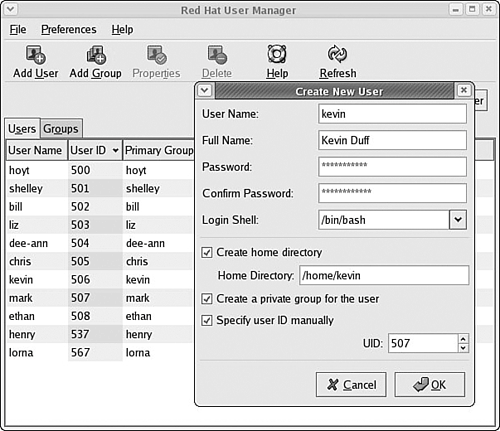
\includegraphics[width=0.8\textwidth]{../imgs/useradd.png}
\end{frame}

\begin{frame}{Group Hug}
\begin{itemize}
\item Why group?
\begin{itemize}
\item Groups establish relationships among users in which they share a common set of permissions
\end{itemize}
\item All the groups are listed in /etc/group file.
\item Group Management Tools:
\begin{itemize}
\item Add a new group with the groupadd command.
\item \# groupadd cdrw
\item Change the group ownership of the device to the new group with the chgrp command.
\item \# chgrp cdrw /dev/scd0
\item Add the approved user to the group with the usermod command.
\item \# usermod -G cdrw  shelley
\item Make user shelley the group administrator with the gpasswd command so that she can add new users to the group.
\item \# gpasswd -A shelley
\end{itemize}
\item There is a GUI for group management as well.
\end{itemize}
\end{frame}

\begin{frame}{User Accounts}
\begin{itemize}
\item Most Linuxes uses the /etc/passwd file to hold user account information. Each user, regardless of type, will have a one-line entry of account information stored in the /etc/passwd text file.
\item The superuser is also known by the name root. 
\item User IDs and Group IDs
\item File Permissions
\begin{itemize}
\item chgrp- Changes the group ownership of a file or directory.
\item chown- Changes the owner of a file or directory.
\item chmod- Changes the access permissions of a file or directory.
\end{itemize}
\end{itemize}
\end{frame}

\begin{frame}{chmod}
\begin{itemize}
\item Try ``ls -l''
\end{itemize}
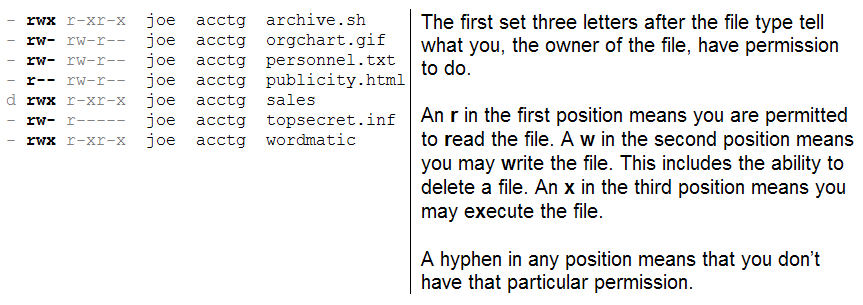
\includegraphics[width=0.8\textwidth]{../imgs/chmod.png}
\begin{itemize}
\item The best way to use chmod is with numbers.  Each permission is assigned a value\\
r = 4, w = 2, x = 1, Therefore:
\begin{itemize}
\item 0: Means no permission
\item 4: Read only
\item 5: Read \& Execute
\item 6: Read \& Write
\item 7: Full permission
\end{itemize}
\end{itemize}
\end{frame}

\begin{frame}{Using chmod}
With chmod you have three numbers: first for the owner, second for group, third for everyone else.\\
Lets do some examples.
\begin{tabular}{| l | l |}
\hline
Before: & -rwxr-xr-x  archive.sh \\ \hline
Command: & chmod 754 archive.sh \\ \hline
After: & -rwxr-xr-- archive.sh \\
\hline
\end{tabular}
\begin{tabular}{| l | l |}
\hline
Before: & -rw-r--r-- topsecret.txt \\ \hline
Command: & chmod 600 topsecret.txt \\ \hline
After: & -rw------- topsecret.txt \\
\hline
\end{tabular}
\begin{tabular}{| l | l |}
\hline
Before: & -rw-------  publicity.html  \\ \hline
Command: & chmod 665 publicity \\ \hline
After: & -rw-rw-r--  publicity.html \\
\hline
\end{tabular}
\end{frame}

\begin{frame}{}
\begin{itemize}
\item The password file is /etc/passwd, and it is the database file for all users on the system. The format of each line is as follows:\\
username:password:uid:gid:gecos:homedir:shell\\
\item Example:
\begin{itemize}
\item sshd:x:74:74:Privilege-separated SSH:/var/empty/sshd:/sbin/nologin
\item rpc:x:32:32:Portmapper RPC user:/:/sbin/nologin
\item rpcuser:x:29:29:RPC Service User:/var/lib/nfs:/sbin/nologin
\item nfsnobody:x:65534:65534:Anonymous NFS User:/var/lib/nfs:/sbin/nologin
\item mailnull:x:47:47::/var/spool/mqueue:/sbin/nologin
\end{itemize}
\end{itemize}
\end{frame}

\begin{frame}{Become Root!}
\begin{itemize}
\item Temporarily Changing User Identity with the su Command\\
\$ su - root
\end{itemize}
\end{frame}

\begin{frame}{Login Process}
\begin{itemize}
{\footnotesize
\item Login prompts for a username.
\item If the /etc/nologin file exists and the user isn't root, a warning message is issued and the login process is halted. The /etc/nologin file is typically used when the system will be shut down shortly and new logins should be restricted.
\item The /etc/usertty file is examined to see if any restrictions are specified for the user. As a security measure, root logons can be restricted to specific terminals and regular users can have the same restrictions placed on them as necessary.
\item The system prompts for a password; it is checked against the encrypted password kept in /etc/shadow. Unsuccessful attempts are logged via the syslog facility and can be reviewed with the lastd command.
\item The user's command shell is started at this point, presenting the user with a command prompt. If no shell is specified for the user in /etc/passwd, /bin/sh is used by default. (Some UNIX operating systems will just log you back out.) If no home directory is specified in /etc/passwd, / is used.
}
\end{itemize}
\end{frame}

\begin{frame}{Quota}
\begin{itemize}
\item Why quota?
\item Disk quotas are designed to control the amount of disk space a user has access to. 
\item Sysadmins use the family of quota commands, such as quotacheck to initialize the quota database files, edquota to set and edit user quotas, setquota to configure disk quotas, and quotaon or quotaoff to control the service. (Other utilities include warnquota for automatically sending mail to users over their disk space usage limit.)
\item man quota
\end{itemize}
\end{frame}

\section{Lab Assignment 01}
\subsection{}
\begin{frame}{}
\begin{itemize}
\item Yes, this is graded.
\item Follow the instructions for lab 01
\end{itemize}
\end{frame}

%\begin{frame}{Event Based Processor}
%\begin{columns}[c]
%\column{0.25\textwidth}
%\begin{block}{OS driven Execution}
    %\includegraphics[width=1.0\textwidth]{imgs/normproc.png}
%\end{block}
%\column{0.25\textwidth}
%\begin{block}{Event Driven Execution}
    %\includegraphics[width=1.0\textwidth]{diagrams/eventproc.png}
%\end{block}
%\column{0.5\textwidth}
%\begin{itemize}
    %\item Normal execution: kernel/software driven
    %\item Event based : event driven
    %\item Performance monitoring is event based
    %\item Next task based on event not scheduled by kernel
    %\item 5.92 times speedup for control dominated programs
%\end{itemize}
%\end{columns}
%\end{frame}

\end{document}
